\chapter{Quantenmechanik}

\section{Grundlagen}

\begin{enumerate}[i)]
	\item \textbf{Wellenfunktion} $ \Psi(\vec{r}) $ $ \qquad $ mit $ \vec{r} $ der \textbf{Ortsdarstellung}
	\begin{equation*}
	P = \int_{V} \left|\Psi ( \vec{r})\right|^2 \dd \vec{r} \quad \tx{Wahrscheinlichkeit} \qquad \quad \int_{V} \left|\Psi(\vec{r})\right|^2 \dd \vec{r} = 1 \quad \tx{Normierungsbedingung}
	\end{equation*}
	\item \textbf{Operatoren} $ \hat{O} $
	\begin{equation*}
	\hat{O} \Psi(\vec{r}) = \Psi'(\vec{r})
	\end{equation*}
	Korrespondenzprinzip
	\begin{align*}
	\vec{r} &= \hat{\vec{r}} \qquad \hat{\vec{r}} \Psi(\vec{r}) = \Psi'(\vec{r}) = \vec{r} \Psi(\vec{r}) \qquad \quad ; \quad \rmbox{\hat{x} \Psi(x) = x \Psi(x) = \Psi'(x)} \\
	\vec{p} &= \hat{\vec{p}} \qquad \hat{\vec{p}} \Psi(\vec{r}) = \Psi'(\vec{r}) = - i \hbar \vabla \Psi(\vec{r}) \quad ; \quad \rmbox{\hat{p}_{x} \Psi(x) = - i \hbar \prd{}{x} \Psi(x) = \Psi'(x) }
	\end{align*}
	$ \hat{\ham} = $ Hamiltonian oder Hamilton-Operator. $ \hat{\ham} = \hat{\ham}(\hat{\vec{r}} , \hat{\vec{p}}) $
	\begin{equation*}
	\hat{\ham} = \frac{\hat{p^2}}{2m} + V(\vec{r}) = - \frac{\hbar^2}{2m} \vabla^2 + V(\vec{r})
	\end{equation*}
	\item \textbf{Zeitabhängige Schrödinger Gleichung}
	\begin{equation*}
	\rmbox{i\hbar \prt{}{t} \Psi(\vec{r}, t) = \hat{\ham}  \Psi(\vec{r}, t)}
	\end{equation*}
	Die klassische Energie sieht so aus:
	\begin{equation*}
	E = \frac{p^2}{2m} + V(\vec{r})
	\end{equation*}
	In der QM dann folgendermaßen:
	\begin{equation*}
	\hat{\ham} = \frac{\hat{p}^2}{2m} + V(\vec{r})
	\end{equation*}
	Die \textbf{Zeitunabhängige Schrödinger Gleichung} sieht wie folgt aus:
	\begin{equation*}
	\rmbox{\hat{\ham} \Psi(\vec{r}) = E \Psi(\vec{r})}
	\end{equation*}
	Diese Gleichung ist eine Eingenwertgleichung. Der Hamilton Operator liefert also den Energie-Eingenwert $ E $ und die Eigenzustände $ \Psi(\vec{r}) $.
	
	\subsection*{Stationäre Zustände}
	
	Jeder messbaren Physikalische Größe ist ein Operator $ \hat{O} $ zugeordnet. Bei einer physikalischen Messung wir der \textbf{Erwartungswert} gemessen: $ \langle \hat{O} \rangle = \langle \Psi | \hat{O} | \Psi \rangle $.
	\begin{equation*}
	\langle \hat{O} \rangle = \langle \Psi(\vec{r}) | \hat{O} | \Psi(\vec{r}) \rangle = \int \Psi^*(\vec{r}) \ \ub{ \hat{O} \ \ \Psi(\vec{r}) }_{\Psi'(\vec{r})} \dd \vec{r}
	\end{equation*}
	\begin{equation*}
	\langle \hat{O}(t) \rangle = \langle \Psi(\vec{r},t) | \hat{O} | \Psi(\vec{r},t) \rangle = \int \Psi^*(\vec{r},t) \hat{O} \Psi(\vec{r},t) \dd \vec{r}
	\end{equation*}
	Diese Gleichung können wir wie folgt umformen:
	\begin{equation*}
	\Psi(\vec{r},t) = \Psi(\vec{r},t = 0) \ub{e^{- \nicefrac{i E t}{\hbar}}}_{\tx{Phasenfaktor}}
	\end{equation*}
	\begin{align*}
	\langle \hat{O} \rangle &= \int \Psi^*(\vec{r}, t = 0) \cancel{e^{\nicefrac{i E t}{\hbar}}} \hat{O} \Psi(\vec{r}, t = 0) \cancel{e^{- \nicefrac{i E t}{\hbar}}} \dd \vec{r} \\
	&= \int \Psi^*(\vec{r}, t = 0) \hat{O} \Psi(\vec{r} , t = 0) \dd \vec{r} \overset{*}{=} \langle \hat{O}(t = 0) \rangle
	\end{align*}
	$ *: $ wenn $ \hat{O} $ nicht Zeitabhängig ist.\\[5pt]
	\textbf{Stationäre Zustände}
	\begin{equation*}
	i \hbar \prt{}{t} \Psi(\vec{r}, t) = \hat{\ham} \Psi(\vec{r}, t) \qquad \tx{mit} \qquad \Psi(\vec{r},t) e^{- \nicefrac{i E t}{\hbar}} \Psi(\vec{r} ,t = 0)
	\end{equation*}
	\begin{equation*}
	\frac{\partial \Psi}{\Psi} = - i \frac{\hat{\ham}}{\hbar} \partial t
	\end{equation*}
	Lösung der DGL mittels Variablen-Trennung
	\begin{equation*}
	\ln\left[\frac{\Psi(\vec{r},t)}{\Psi(\vec{r}, t = 0)}\right] = - \frac{i \hat{\ham} t}{\hbar} \quad \Rightarrow \quad \Psi(\vec{r}, t) = e^{- \nicefrac{i \hat{\ham} t}{\hbar}} \Psi(\vec{r}, t = 0)
	\end{equation*}
	\begin{equation*}
	\hat{\ham} \Psi(\vec{r} , t = 0) = E \Psi(\vec{r}, t = 0)
	\end{equation*}
	Taylor Entwicklung:
	\begin{equation*}
	e^{x} = e^{- \nicefrac{i \hat{\ham} t}{\hbar}} = a \left(\hat{\ham}\right)^0 + b \left(\hat{\ham}\right)^1 + c \left(\hat{\ham}\right)^2 + \dots
	\end{equation*}
	\begin{align*}
	e^{- \nicefrac{i \hat{\ham} t}{\hbar}} \Psi(\vec{r}, t = 0)&= a \Psi(\vec{r}, t = 0) + b \hat{\ham} \Psi(\vec{r}, t = 0) + c \hat{\ham} \cdot \hat{\ham} \Psi(\vec{r}, t = 0) + \dots \\
	&= a \Psi(\vec{r}, t = 0) + b E \Psi(\vec{r}, t = 0) + c E^2 \Psi(\vec{r}, t = 0) + \dots \\
	&= (a + bE + c E^2 + \dots) \cdot \Psi(\vec{r}, t = 0) \\
	&= e^{- \nicefrac{i E t}{\hbar}} \Psi(\vec{r}, t = 0)
	\end{align*}
	\lcom{Wir können einen Operator in der $ e $-Funktion schreiben, da diese mit der Taylorentwicklung als Reihe entwickelt werden kann.}
	\item \textbf{Spin} (Elektronen)
	\begin{enumerate}[$ \Rightarrow $]
		\item Wasserstoffatom (Stern-Gerlach)
		\item Helium (Pauli Prinzip)
	\end{enumerate}
	\newpage
	\item \textbf{Quantensysteme}
	\begin{itemize}
		\item Freies Teilchen, Potentialstufe (Tunneln)
		\item Harmonischer Oszillator $ \Rightarrow $ Molekülphysik
		\item Coulomb Potential $ \Rightarrow $ Wasserstoffatom
	\end{itemize}
	\begin{figure}[ht]
		\centering
		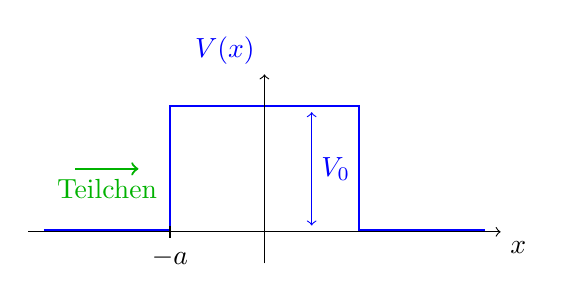
\begin{tikzpicture}[scale=0.8]
		\draw[thick,blue] (-3.5,.025) -| (-1.5,2) -- (1.5,2) |- (3.5,.025);
		\draw[thick,black!30!green,->] (-3,1) -- node[below] {Teilchen} ++(1,0);
		\draw[->] (-3.75,0) -- (3.75,0) node[anchor=north west] {$ x $};
		\draw[->] (0,-0.5) -- (0,2.5) node[anchor=south east] {\color{blue}$ V(x) $};
		\draw (-1.5,.1) -- ++(0,-.2) node[below] {$ -a $};
%		\draw (1.5,.1) -- ++(0,-.2) node[below] {$ +a $};
%		\node[draw=black,circle, minimum size=.8cm,red] at (-2.5,-1) {I};
%		\node[draw=black,circle, minimum size=.8cm,red] at (0,-1) {II};
%		\node[draw=black,circle, minimum size=.8cm,red] at (2.5,-1) {III};
		\draw[<->,blue] (.75,.1) -- node[right] {$ V_0 $} ++(0,1.8); 
		\end{tikzpicture}
		\label{Potentialbarriere}
		\caption{Darstellung einer Potentialbarriere. Beispiel für den Tunneleffekt eines hindurchfliegenden Teilchens, das eigentlich weniger Energie hat als klassisch nötig wäre um die Barriere zu überwinden. Dieses Bild wurde mit dem \LaTeX Paket Tikz erstellt.}
	\end{figure}
	\FloatBarrier
	\item \textbf{Kommutatoren}
	\begin{align*}
	\hat{x}&: \vec{p} = \vec{p}_x \qquad \qquad \left[\hat{x}, \hat{p}\right] = \hat{x} \hat{p} - \hat{p} \hat{x} \\
	\hat{A}; \hat{B}&: \qquad \qquad \qquad \ \left[\hat{A}, \hat{B}\right] = \hat{A} \hat{B} - \hat{B} \hat{A}
	\end{align*}
	Wellenfunktion $ \Psi(x) \qquad \qquad \left[\hat{x}, \hat{p}\right] \Psi(x) = \Psi'(x) $
	\begin{equation*}
	\left[\hat{x}, \hat{p}\right] = \hat{x} \hat{p} - \hat{p} \hat{x} = x \left(- i \hbar \prd{}{x}\right) - \left(- i \hbar \prd{}{x}\right) x
	\end{equation*}
	\begin{align*}
	\left[\hat{x}, \hat{p}\right] \Psi(x) &= \left\{ x \left(- i \hbar \prd{}{x}\right) - \left(- i \hbar \prd{}{x}\right) x \right\} \Psi(x) \\
	&= x \left(- i \hbar \prd{}{x} \Psi(x) \right) - \left(- i \hbar \prd{}{x}\right) x \Psi(x) \\
	&= - i \hbar x \prd{\Psi}{x} + i \hbar \prd{}{x} ( x \Psi(x)) \\
	&= \cancel{ - i \hbar x \prd{\Psi}{x}} \cancel{+ i \hbar x \prd{\Psi}{x}} + i \hbar \Psi(x) \ub{\prd{x}{x}}_{=1} \\
	&= i \hbar \Psi(x) = \Psi'(x)
	\end{align*}
	\begin{equation*}
	\rmbox{\left[\hat{x}, \hat{p}\right] = i \hbar} \quad \Rightarrow \quad \tx{die zwei Operatore vertauschen nicht !!!}
	\end{equation*}
	
	\subsection*{Eigenschaft Kommutator}
	
	$ \hat{A} $; $ \hat{B} $
	\begin{equation*}
	\Delta A \cdot \Delta B \ge \frac{1}{2} \left| \langle \left[\hat{A}, \hat{B}\right] \rangle \right|
	\end{equation*}
	$ \left[\hat{A}, \hat{B}\right] $ Operator $ \Rightarrow $
	\begin{align*}
	\langle \left[\hat{A}, \hat{B}\right] \rangle &= \langle \hat{A} \hat{B} - \hat{B} \hat{A} \rangle \\
	&= \langle \Psi | \hat{A} \hat{B} - \hat{B} \hat{A} | \Psi \rangle \\
	&= \int \Psi^* \left(\hat{A} \hat{B} - \hat{B} \hat{A}\right) \Psi \dd \vec{r}
	\end{align*}
	$ \Delta A $, $ \Delta B $ Standardabweichung
	\begin{equation*}
	\sigma_x = P(x) \quad \sigma_x = \left[ \int (x - \mu)^2 P(x) \dd x \right]^{1/2}  \qquad \mu = \int x P(x) \dd x
	\end{equation*}
	
	% T Gaußglocke
	
	\begin{figure}
		\centering
		\begin{tikzpicture}
			\draw[->] (0,-0.2) -- (0,2.5) node[anchor=south east] {$ P(x) $};
			\draw[->] (-0.2,0) -- (7,0) node[anchor=north west] {$ x $};
			\draw[domain=0:7, samples=80, thick] plot (\x, {2*exp(-(\x - 3.5)^(2)*0.6});
			\coordinate (o) at (3.5,1);
			\coordinate (d) at (1.1,0);
			\draw[ultra thick, <->, blue, arrows = {Stealth}-{Stealth}] ($ (o) + (d) $) -- ($ (o) - (d) $);
		\end{tikzpicture}
		\label{Gausverteilung}
		\caption{Die Wahrscheinlichkeitsverteilung einer Gaußkurve. Der Pfeil soll die Standartabweichung darstellen. Dieses Bild wurde mit dem \LaTeX Paket Tikz erstellt.}
	\end{figure}
	
	$ \hat{A} = \hat{x} $, $ \hat{B} = \hat{p} $. $ \left[\hat{x}, \hat{p}\right] = i \hbar $
	\begin{equation*}
	\Delta A \cdot \Delta B \ge \frac{1}{2} \left| \langle \left[\hat{A}, \hat{B}\right] \rangle \right|
	\end{equation*}
	\begin{equation*}
	\Delta x \cdot \Delta p \ge \frac{1}{2} \left| i \hbar \right| = \frac{\hbar}{2}
	\end{equation*}
	
	\subsection*{Morgen:}
	
	Operatoren die vertauschen: Drehimpulsoperator $ \vec{l} $ mit den Komponenten $ l_x, l_y, l_z $ und $ l^2 $. Es gilt $ \left[l^2, l_z\right] = 0 $
	\begin{equation*}
	\Delta l^2 \cdot \Delta l_z \ge 0
	\end{equation*}
	Man kann also Zustände finden, bei denen $ \Delta l^2 = 0 $; $ \Delta l_z = 0 $ sind. Diese Zustände können im Prinzip existieren und verletzen die Unschärferelation nicht! Diese Zustände sind dann gleichzeitig Eigenzustände von $ l^2 $ und $ l_z $.
	
	\subsubsection*{Exkurs: Varianz und Standardabweichung in der Quantenmechanik}
	
	Wellenfunktion $ \Psi(x) $ mit Wahrscheinlichkeit $ P(x) = |\Psi(x)|^2 $
	\begin{align*}
	\mu &= \int x P(x) \dd x = \int x | \Psi(x) | ^2 \dd x \\
	\sigma   &= \int x^2 P(x) \dd x = \int x^2 | \Psi(x) | ^2 \dd x
	\end{align*}
	Die Varianz ist definiert als:
	\begin{align*}
	\sigma^2 = \int (x - \mu)^2 P(x) \dd x &= \int (x^2 + \mu^2 - 2 \mu x) P(x) \dd x \\
	&= \int x^2 P(x) \dd x + \mu^2 \int P(x) \dd x - 2 \mu \int x P(x) \dd x\\
	&= \int x^2 P(x) \dd x + \mu^2 - 2 \mu \mu = \int x^2 P(x) \dd x - \mu^2 \\
	&= \langle x ^2 \rangle - \langle x \rangle ^2
	\end{align*}
	
\end{enumerate}
